\documentclass[10pt]{beamer}
\usepackage{verbatim}
\usepackage{amsmath}
\usepackage{amsthm}
\usepackage{graphics}
\usepackage{color}
\usepackage{algorithm, algorithmic}
\usepackage{stmaryrd}\usefonttheme[onlymath]{serif}

\title{Discussion 3: Algorithm V1 \& Experiment on Cases}
\begin{document}

\maketitle
\begin{frame}\frametitle{Algorithm Version 1}
\begin{algorithm}[H]
\caption{Algorithm Version1: Learn Multiphase RF Incrementally}
\begin{algorithmic}[1]
\REQUIRE Loop $L$, depthBound $db$

\ENSURE $\texttt{result}\in \{\texttt{FIN, INF, UNKNOWN}\}$, a list of RFs \texttt{rf\_list}
\STATE $i := 0, \texttt{result} := \texttt{UNKNOWN},\texttt{rf\_list} := []$
\WHILE{$i < db$ and \texttt{result}$ == \texttt{UNKNOWN}$}
\STATE \texttt{result}, \texttt{rf} $ = $ \texttt{LearnRankerBounded}$(L)$
\IF{$\texttt{result} == \texttt{INF}$ or $\texttt{result} == \texttt{FIN}$}
\STATE $\texttt{rf\_list.append(rf)}$
\STATE $\texttt{return result, rf\_list}$
\ELSE 
\STATE \texttt{result}, \texttt{rf} $ = $ \texttt{LearnRankerNoBound}$(L)$
\STATE \texttt{rf\_list.append(rf)}
\ENDIF
\STATE $L = $ \texttt{ConjunctConstraint($L$, rf)}
\STATE $i \texttt{+=} 1$
\ENDWHILE
\STATE \texttt{return UNKNOWN, rf\_list}
\end{algorithmic}
\end{algorithm}
\end{frame}


\begin{frame}\frametitle{Case 1: Multiphase}
\begin{example}
\texttt{while($x$ > 0 or $y$ > 0) do }$x' = x + y - 1; y' = y - 1$

is a loop ranked by 2-phase multiphase ranking function: $\langle y, x\rangle$
\end{example}

Result of the algorithm: $\langle 0.9971 y, 0.639x + 0.6774\rangle$

\begin{center}
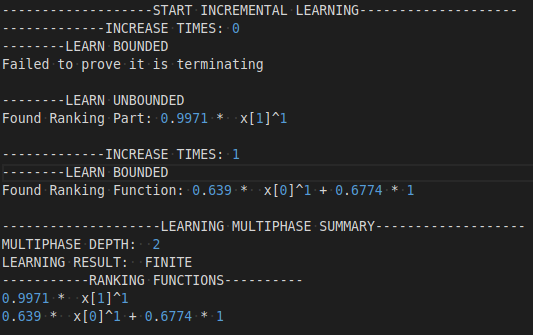
\includegraphics[scale=0.5]{1.png}
\end{center}

\end{frame}

\begin{frame}\frametitle{Case 2: Multiphase plus Branch}
\begin{example}
\texttt{while($x$ > 0 or $y$ > 0) do }

$\texttt{If y > 0:} x' = x; y' = y - 1;$
$\texttt{else:} x' = x - 1; y' = y;$


\end{example}

is a loop with 2-phase multiphase ranking function $\langle y, x\rangle$

Use template $ax + by + c$ to run:
\begin{center}
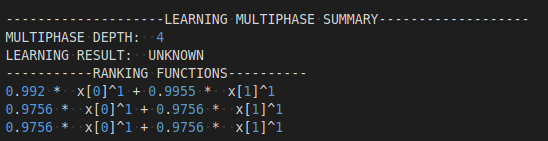
\includegraphics[scale= 0.5]{2.png}
\end{center}
where the learn unbound part always generating $x + y$ as a decreasing function.

\end{frame}

\begin{frame}\frametitle{Way to solve the problem}
Try a different template when learning failed.

If we try $by + c$ as the first template and $ax + by + c$ as the second:

\begin{center}

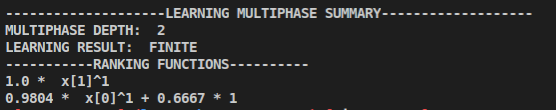
\includegraphics[scale= 0.5]{3.png}
\end{center}

We have to modify our algorithm to by adding back-tracking to try different template when we fail to learn a ranking function out. 
\end{frame}

\begin{frame}\frametitle{Case 3: Multiphase Nested-RF}
\begin{example}
\texttt{while($x$ > 0 or $y$ > 0) do }$x' = x + y; y' = y - 1$

This is a false example for multiphase ranking function $\langle y,x\rangle$ for when $y < 0$ 
\[ x - x' = -y > 0\]

not $\delta$.



\end{example}

\end{frame}


\end{document}